\section{Preventivo}
\par Il preventivo viene formulato tenendo in considerazione il costo orario di ciascun ruolo, il budget stimato e le attività pianificate per il periodo corrispondente. Ogni \glossario{sprint} è corredato da:
\begin{itemize}
    \item Un preventivo orario in forma tabellare;
    \item Un areogramma della distribuzione oraria per la coppia risorsa-ruolo;
    \item Un preventivo economico in forma tabellare;
    \item Un istogramma della distribuzione oraria per ruolo.
\end{itemize}

\vspace{0.5\baselineskip}
\par Il rendimento complessivo per ciascun componente è di 91 ore, ripartite equamente nei ruoli di progetto, per un totale di 637 ore produttive. L'uniformità nella distribuzione dei ruoli tra i membri del team viene mantenuta procedendo a rotazione, affinché ogni risorsa possa esplorare tutte le mansioni. Al fine di migliorare la leggibilità e la compattezza delle tabelle, i ruoli di progetto sono identificati dalle seguenti \glossario{abbreviazioni}: 
\begin{itemize}
    \item \textbf{Re}: Responsabile;
    \item \textbf{Am}: Amministratore;
    \item \textbf{An}: Analista;
    \item \textbf{Pt}: Progettista;
    \item \textbf{Pr}: Programmatore;
    \item \textbf{Ve}: Verificatore.
\end{itemize}

%\subsection{RTB}
%TODO
\subsubsection{Sprint 1: da 2024-04-03 a 2024-04-19}
\begin{minipage}{\textwidth}
Di seguito è riportata la distribuzione delle ore per ciascun membro del team, accumulate in totali per persona e per ruolo:
\begin{table}[H]
  \begin{tabularx}{\textwidth}{|c|*{6}{>{\centering}X|}c|}
    \hline
    \multicolumn{8}{|c|}{\textbf{Preventivo orario}} \\
    \hline
    \textbf{Membro del team} & \textbf{Re} & \textbf{Am} & \textbf{An} & \textbf{Pt} & \textbf{Pr} & \textbf{Ve} & \textbf{Totale per persona} \\
    \hline
    Cavalli Riccardo & 7 & 0 & 0 & 0 & 0 & 0 & 7 \\
    \hline
    Pianon Raul & 0 & 0 & 0 & 0 & 0 & 8 & 8 \\
    \hline
    Dall'Amico Martina & 0 & 0 & 9 & 0 & 0 & 0 & 9 \\
    \hline
    Cristo Marco & 0 & 0 & 9 & 0 & 0 & 0 & 9 \\
    \hline
    Lewental Sebastiano & 0 & 0 & 9 & 0 & 0 & 0 & 9 \\
    \hline
    Zecchinato Mattia & 0 & 0 & 0 & 7 & 0 & 0 & 7 \\
    \hline
    Stocco Tommaso & 0 & 6 & 0 & 0 & 0 & 0 & 6 \\
    \hline
    \textbf{Totale per ruolo} & 7 & 6 & 27 & 7 & 0 & 8 & \textbf{55} \\
    \hline
  \end{tabularx}
  \caption{Sprint 1 - Preventivo orario}
\end{table}
\end{minipage}

\begin{figure}[H]
  \centering
  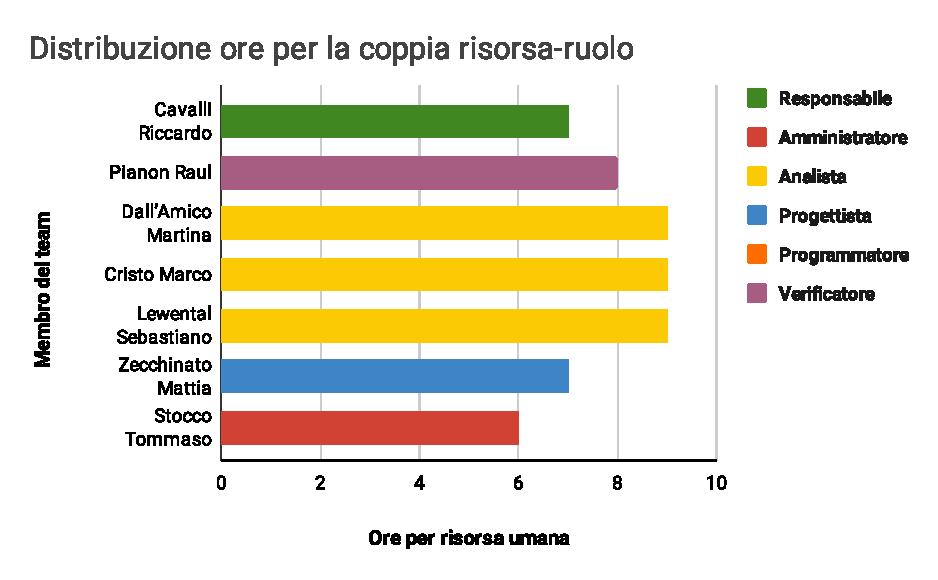
\includegraphics[width=0.90\textwidth]{assets/Preventivo/Sprint-1/distribuzione_ore_risorsa_ruolo.pdf}
  \caption{Sprint 1 - Istogramma della distribuzione oraria per la coppia risorsa-ruolo}
\end{figure}

\begin{figure}[H]
  \centering
  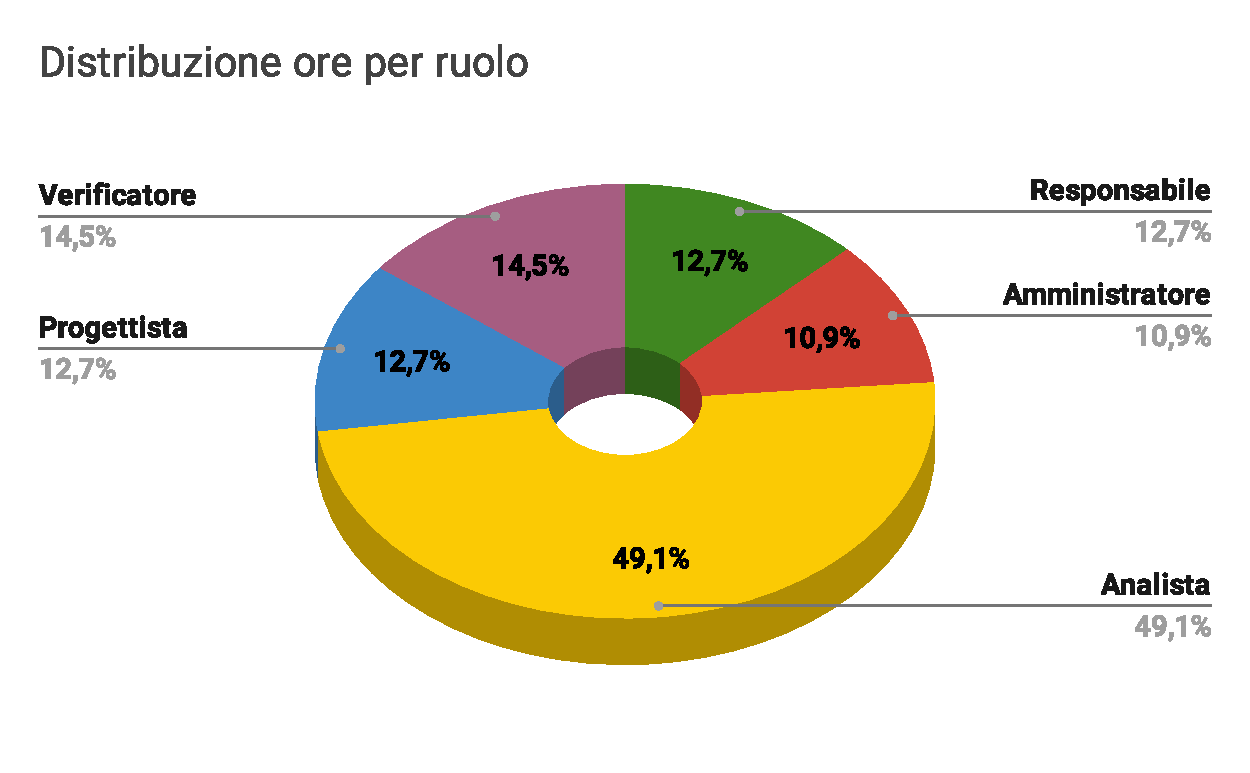
\includegraphics[width=0.90\textwidth]{assets/Preventivo/Sprint-1/distribuzione_ore_ruolo.pdf}
  \caption{Sprint 1 - Areogramma della distribuzione oraria per ruolo}
\end{figure}

Di seguito è riportato il preventivo economico del primo \glossario{sprint}:
\begin{table}[H]
  \centering
  \begin{tabular}{|c|c|c|}
    \hline
    \multicolumn{3}{|c|}{\textbf{Preventivo economico}} \\
    \hline
    \textbf{Ruolo} & \textbf{Ore per ruolo} & \textbf{Costo (in \texteuro)} \\
    \hline
    Responsabile & 7 & 210,00 \\
    \hline
    Amministratore & 6 & 120,00 \\
    \hline
    Analista & 27 & 675,00 \\
    \hline
    Progettista & 7 & 175,00 \\
    \hline
    Programmatore & 0 & 0,00 \\
    \hline
    Verificatore & 8 & 120,00 \\
    \hline
    \textbf{Totale} & 55 & \textbf{1.300,00} \\
    \hline
  \end{tabular}
  \caption{Sprint 1 - Preventivo economico}
\end{table}